\section[Проектирование приложения]{%
  ПРОЕКТИРОВАНИЕ ПРИЛОЖЕНИЯ
}

\label{sec:design}

% Общая характеристика задачи

\subsection{Общая характеристика задачи}

Объектом проектирования является мобильное приложение,
отображающее актуальную информацию о курсах валют в Республике Беларусь.

Мобильное приложение является самостоятельной программной единицей,
может быть установлено на iPhone с
использованием магазина приложений от Apple App Store.

В качестве входной информации для приложения выступают два интернет-ресурса.

Первый интернет ресурс предоставляет данные о курсах валют, выставленных
национальным банком Республики Беларусь на текущую дату,
получаемых в формате JSON по определённому GET-запросу.

Второй интернет ресурс предоставляет адресно-справочную информацию,
курсы обмена валют в отделениях коммерческих банков в формате XML. Запрос
является параметрическим, в качестве параметра выступает идентификатор
областного центра. Таким образом, имеется возможность получить информацию
об отделениях для заданного областного центра. Стоит отметить, что этот запрос
выполняется с использованием базовой HTTP-аутентификацией, то есть доступ
к ресурсу возможен только при наличии логина и пароля.

Выходной информацией является обработанная и предоставленная в удобном для
пользователя виде информация об отделениях банков, курсов валют в них,
а также о курсе валют, установленном национальным банком Республики Беларусь.

Целью установки приложения для пользователей может стать желание знать о
результатах проведения торгов на белорусской валютно-фондовой бирже,
интерес к актуальным ценам на валюты в отделениях коммерческих банков
Республики Беларусь, или же получение адресно-справочной информации о банках.
Таким образом сценариями использования приложения могут стать:
\begin{itemize}
  \item просмотр курсов валют;
  \item просмотр адресно-справочной информации;
  \item использование конвертер валют;
  \item выполнение поиска отделений по адресу, названию банка;
  \item изменение выбранной валюты;
  \item изменение областного центра.
\end{itemize}

Стоит заметить, что некоторые сценарии использования можно сгруппировать.
Например, просмотр курсов валют и просмотр адресно-справочной информации можно
объединить таким образом, что просмотр детальной информации об отделении будет
расширять просмотр списка отделений с курсами обмена валют в этих отделениях.

Окончательная диаграмма прецедентов приложения
представлена на рисунке~\ref{fig:use_case}.
\begin{figure}[h!]
  \centering
  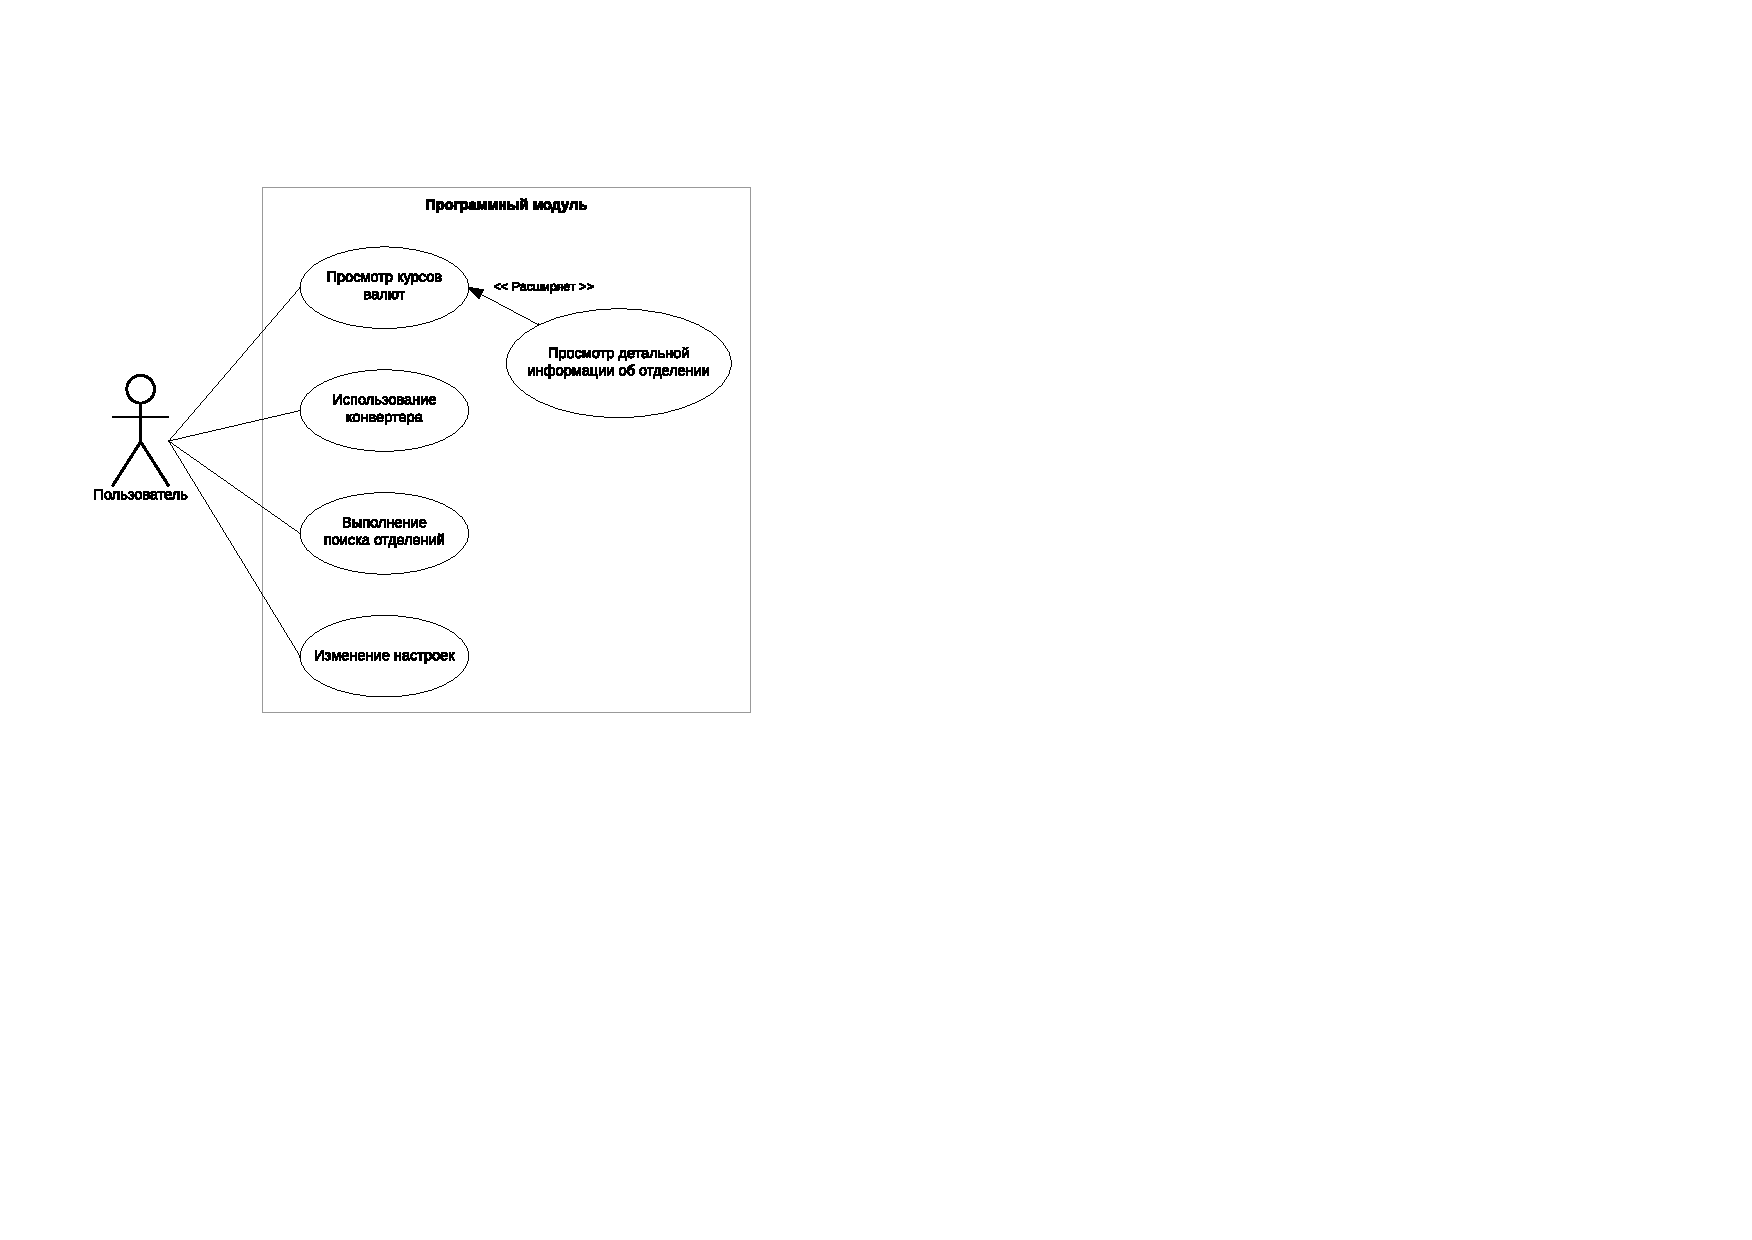
\includegraphics[width=140mm]{fig/use_case}
  \caption{Диаграмма прецедентов приложения}
  \label{fig:use_case}
\end{figure}

Поскольку при разработке программного модуля ставится цель сделать его
максимально независимым от подключения к интернету, то очевидным становится
необходимость использования мобильного хранилища данных. Для лучшей
структурированности информации, а также достижения высокой скорости работы приложения,
в качестве хранилища данных следует использовать мобильную базу данных.

\pagebreak


% Возможно: Взаимодействие программного модуля с внешней средой
% Внешняя архитектура программного модуля

\subsection{Внешняя архитектура программного модуля}

Большинство мобильных приложений построены и с использованием клиент-серверной
архитектуры, в которой сервером данных может выступать сторонний API-сервис.

Архитектура <<клиент-сервер>> представляет собой вычислительную архитектуру,
где задачи и сетевая нагрузка распределены между программным обеспечением,
которое является поставщиком ресурсов и услуг --- сервером и заказчиком ресурсов
и услуг --- клиентом.
Сервер представляет собой хранилище данных и предоставляет доступ к этим
данным другим объектам сети по их запросам.
Клиент --- это рабочая станция, которая использует ресурсы сервера и
предоставляет пользователю удобный интерфейс для управления этими ресурсами.
Клиент не должен иметь непосредственных связей с базой данных для
обеспечения безопасности данных и быть нагруженным основной логической
составляющей приложения для возможного осуществления масштабируемости системы.
Сервер работает по запросам клиентов и управляет обработкой этих запросов.
После выполнения каждого запроса, вне зависимости от результата обработки,
сервер отправляет ответ клиенту, пославшему этот запрос.
Обычно клиент и сервер располагаются на разных вычислительных машинах,
но могут выполняться также и на одной машине.

Разрабатываемый программный модуль представляет собой клиентское приложение,
которое с использованием HTTP-запросов общается с двумя удалёнными серверами данных.
Используемая архитектура разрабатываемого приложения продемонстрирована
на рисунке~\ref{fig:client_servers_schema}.
\begin{figure}[h!]
  \centering
  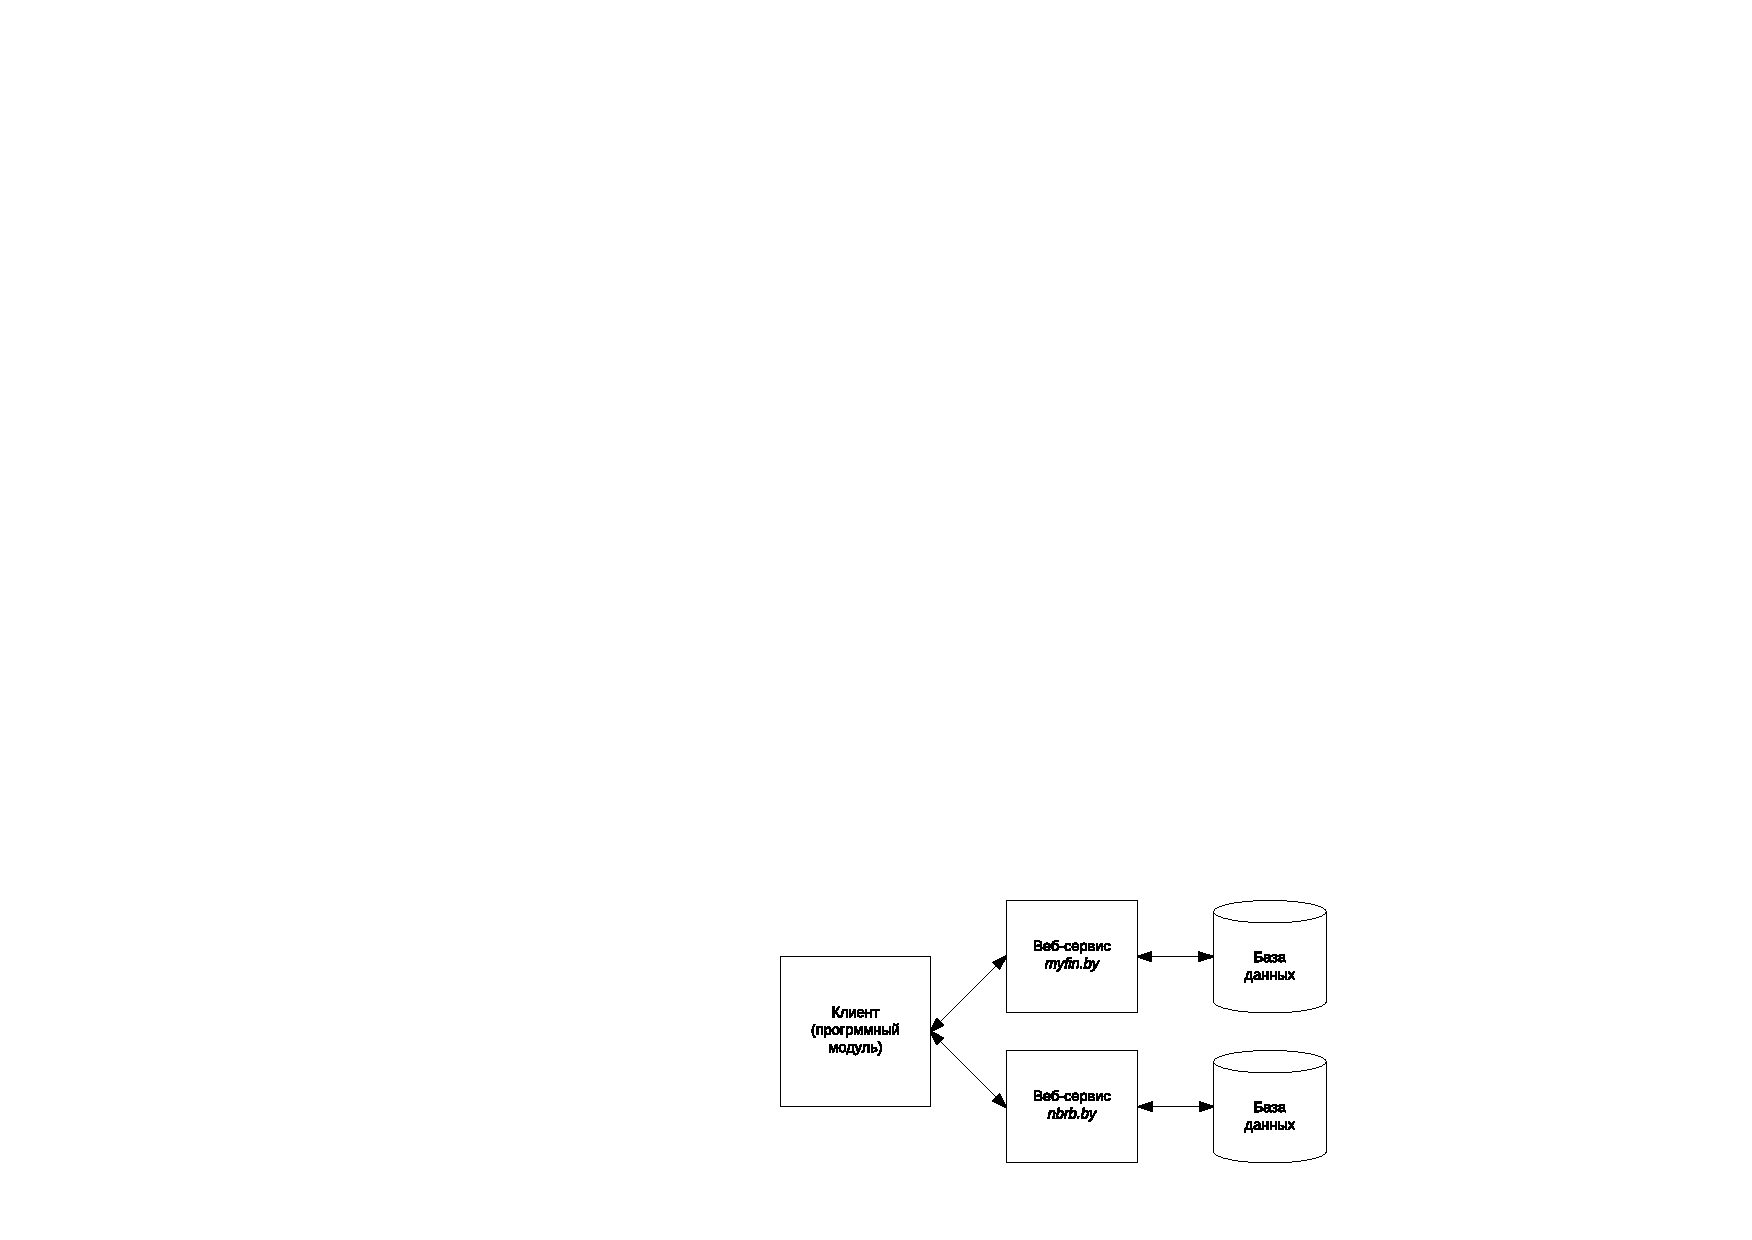
\includegraphics[width=110mm]{fig/client_servers_schema}
  \caption{Клиент-серверная архитектура разрабатываемого программного модуля}
  \label{fig:client_servers_schema}
\end{figure}


% Внутренняя архитектура программного модуля

\subsection{Внутренняя архитектура программного модуля}

Большим плюсом в создании программных продуктов является следование некоторому
паттерну проектирования. Шаблоны упрощают повторное использование удачных
архитектурных и проектных решений.
Кроме того, с помощью паттернов можно существенно
упростить процесс сопровождения разработанных систем и улучшить
качество документации, позволяя явно описать функции тех или иных
классов и объектов, а также взаимодействие между ними.

Рассмотрим различные подходы к проектированию мобильных приложений на платформе
iOS с точки зрения архитектуры.


% MVC

\paragraph{}

Паттерн Model-View-Controller (англ. Модель-Представление-Контроллер) представляет
собой шаблон проектирования, согласно которому модель данных,
пользовательский интерфейс и механизм взаимодействия с пользователем разделены
на три отдельных компонента, специализирующихся на своих задачах.
Таким образом, изменение одного из компонентов не оказывает существенного
влияния на остальные, и приложения, построенные согласно концепции MVC,
расширяются легче, чем другие приложения.
Схема взаимодействия элементов шаблона проектирования MVC
представлена на рисунке~\ref{fig:mvc}.
\begin{figure}[h!]
  \centering
  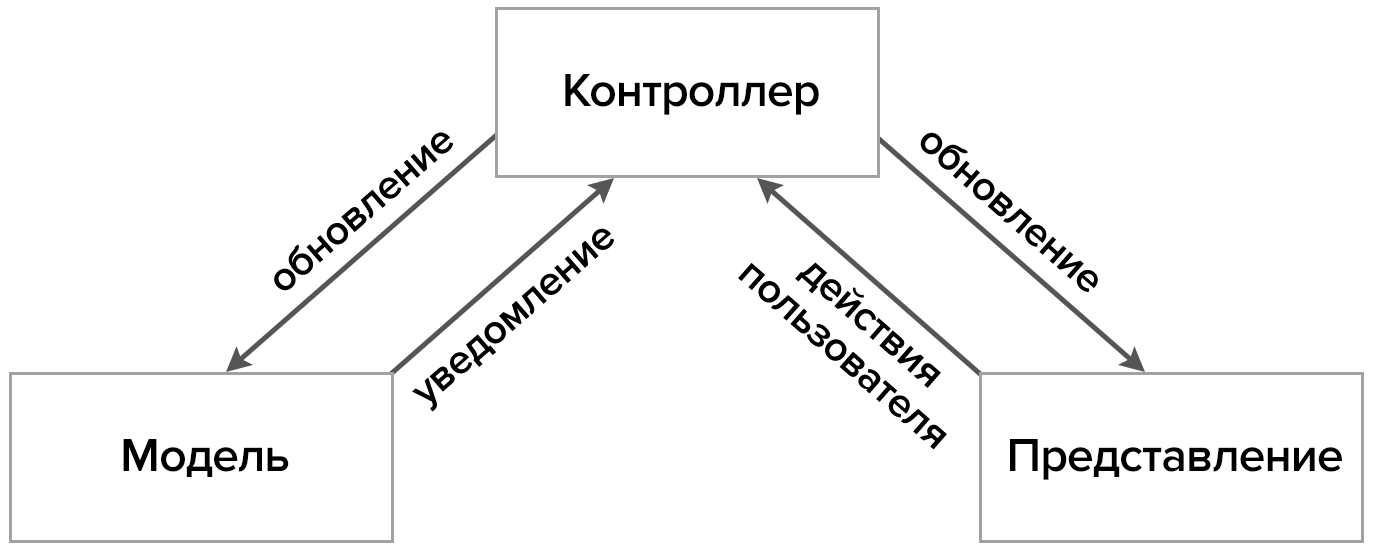
\includegraphics[width=140mm]{fig/mvc}
  \caption{Схема шаблона проектирования MVC}
  \label{fig:mvc}
\end{figure}

Модель (англ. <<Model>>), согласно концепции MVC, содержит данные приложения и определяет правила,
принципы и зависимости поведения этих данных. Например, объект модели может
представлять собой персонаж игры или контакт в адресной книге.
Объект модели может иметь связи один-к-одному или один-ко-многим с другими
объектами модели и быть связан с одним или более объектами представления.

Представление (англ. <<View>>) включает в себя элементы приложения,
которые может видеть пользователь, а именно элементы пользовательского интерфейса.
Основная цель объектов представления --- отображение данных объектов модели приложения
и предоставление инструментов для редактирования этих данных.

Контроллер (англ. <<Controller>>) выступает в качестве посредника между одним или
несколькими объектами представления и одним или несколькими объектами модели.
Объекты поведения являются каналом, через которые объекты представления
узнают об изменениях в объектах модели и наоборот~\cite{mvc_apple_docs}.


% MVVM

\paragraph{}

Приложения для платформы iOS, созданные с использованием архитектуры
Model-View-ViewModel (англ.~Модель-Представление-Модель Представления),
стали появляться относительно недавно. Изначально, этот паттерн использовался
исключительно в некоторых продуктах корпорации Microsoft. Желание использовать
MVVC у разработчиков зачастую возникает в связи с необходимостью
обновлением компонента <<Представление>> вручную, то есть каждый раз, когда
что-либо обновляется в объекте модели, разработчику необходимо вручную
обновить отображаемую информацию.

Паттерн MVVM лишен этого недостатка, так как гарантирует полное
соответствие объекта представления (то есть того, что отображается пользователю) тому,
что хранится в объекте <<Модель Представления>>.
Взаимодействие базовых элементов архитектуры Model--View--ViewModel
представлено на рисунке~\ref{fig:mvvm}.
\begin{figure}[h!]
  \centering
  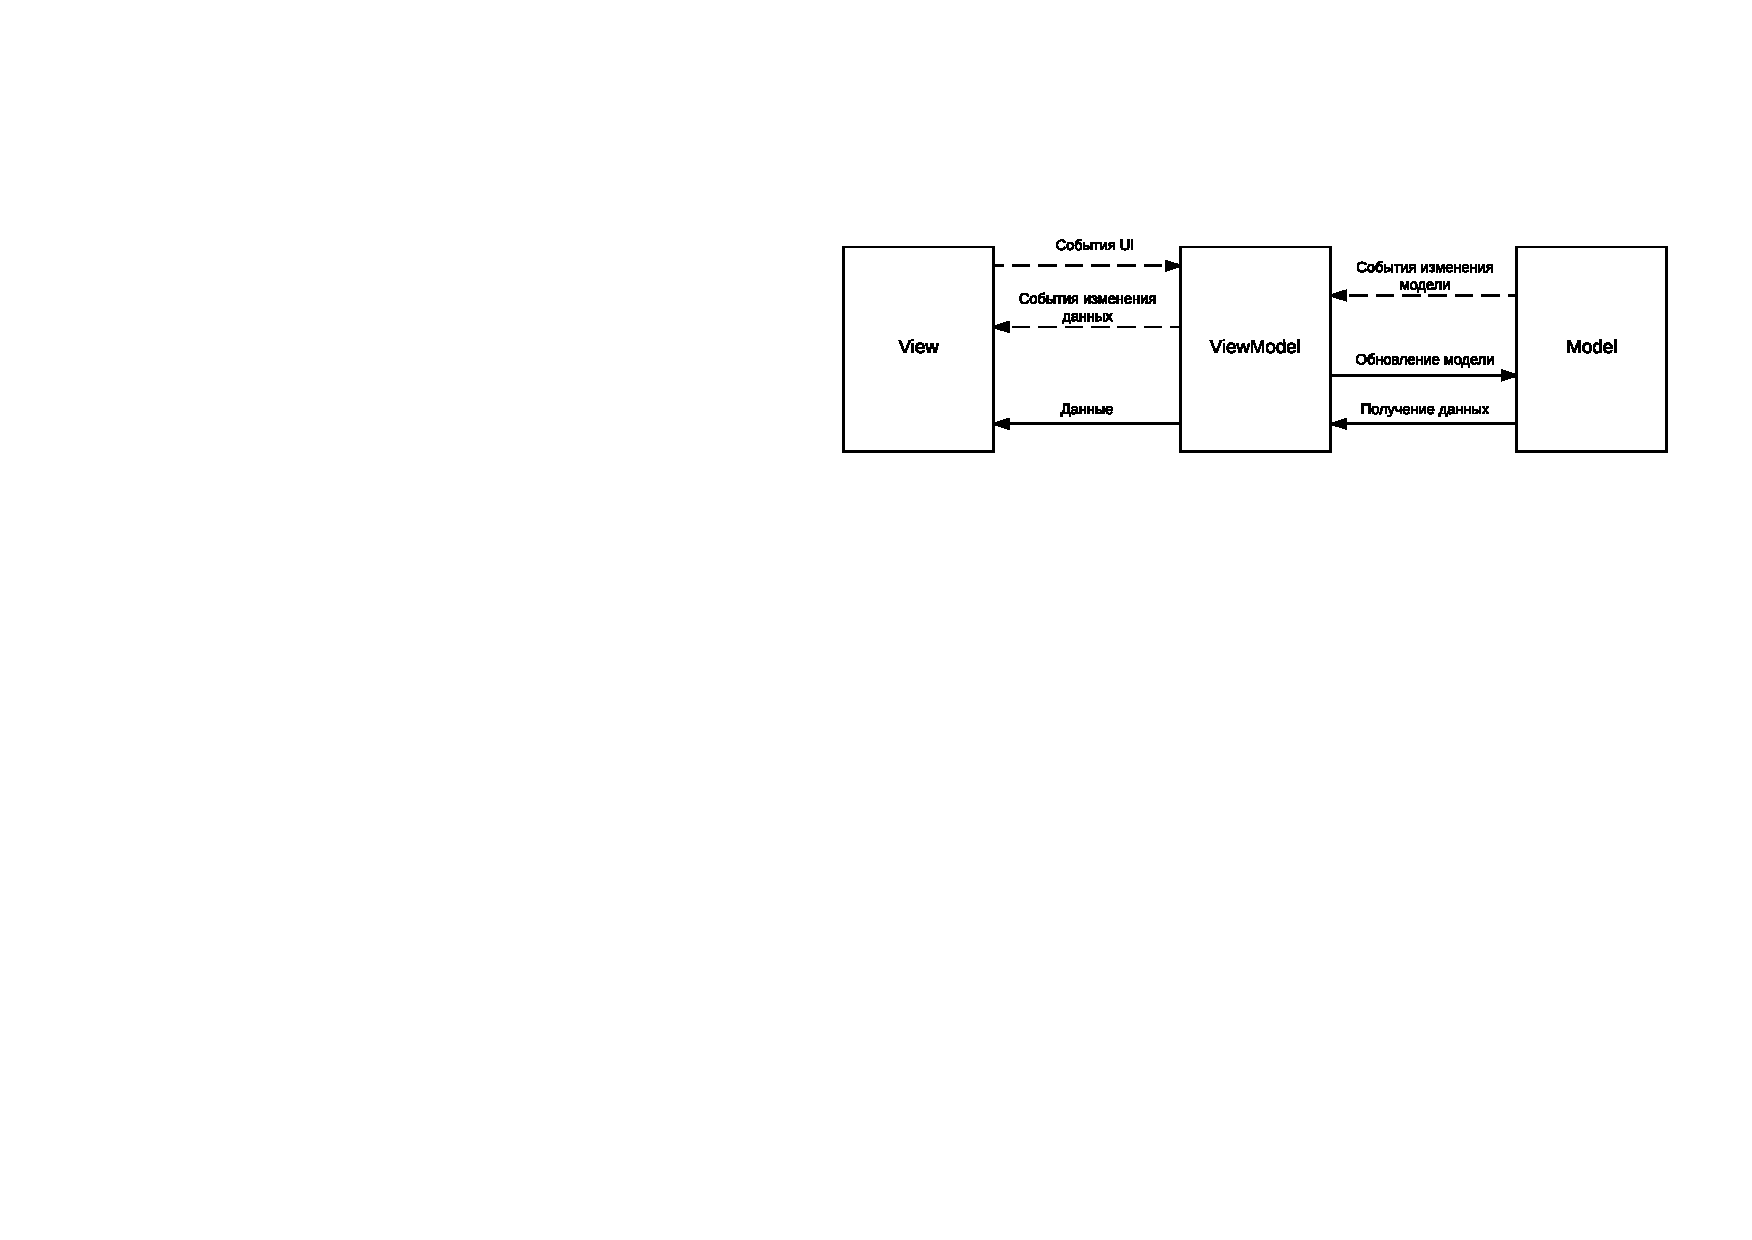
\includegraphics[width=140mm]{fig/mvvm}
  \caption{Схема шаблона проектирования MVVM}
  \label{fig:mvvm}
\end{figure}

\pagebreak

% VIPER

\paragraph{}

Развитие архитектуры создания мобильных приложений VIPER начинается
с момента публикации статьи на известном среди iOS-разработчиков
интернет-портале objc.io~\cite{viper_objc_io}.

Толчком для написания этой статьи, в свою очередь,
стала статья <<The Clean Architecture>>~\cite{clean_architecture},
в которой Роберт Мартин изложил основные принципы разделения логической
структуры приложения на уровни обязанностей. Такой подход может
существенно упростить изолирование зависимостей и тестирование взаимодействий
на границах между уровнями.

В результате архитектура VIPER представляет собой реализацию
изложенного в статье Роберта Мартина подхода к разработке программного обеспечения
для конкретной платформы --- iOS. Слово VIPER является бэкронимом для View,
Interactor, Presenter, Entity и Routing. Для каждого элемента этой архитектуры
предполагается создание отдельного файла. Взаимодействие элементов архитектуры
VIPER представлено на рисунке~\ref{fig:viper}.
\begin{figure}[h!]
  \centering
  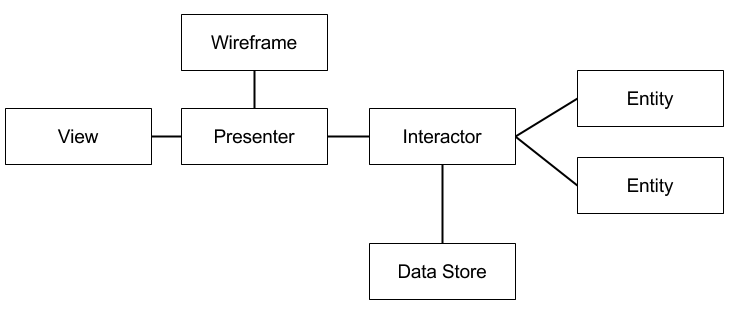
\includegraphics[width=150mm]{fig/viper}
  \caption{Взаимодействие элементов архитектуры VIPER}
  \label{fig:viper}
\end{figure}

Интерактор (англ. Interactor) содержит бизнес-логику для управления объектами,
чтобы выполнить определённую задачу. Любая задача выполняется в интеракторе независимо
от слоя представления, то есть один и тот же интерактор можно использовать как в
создании мобильных приложений, так и для консольных программных модулей для OS X.

Сущности (англ. Entities) --- объекты, которыми управляет слой <<Интерактор>>.

В элементе <<Презентатор>> (англ. Presenter) содержится логика управления слоем
отображения информации пользователю. Этот элемент также получает результаты
интерактора и преобразовывать результаты в состояние, которое является наиболее
эффективным для отображения пользователю.

Вид (англ. View) является пассивным элементом структуры, который ожидает уведомлений
со стороны презентатора для вызова методов отображения данных пользователю.

Каркас (англ. Wireframe) отвечает как за сборку всего модуля (логическое
соединение всех элементов), так и за переходы (навигацию) между экранами
в приложении.

Благодаря использованию архитектуры VIPER разработчикам удаётся
разделять большое количество кода одного класса на несколько меньших классов,
что может существенно упростить разработку классов приложения,
разделить обязанности членов команды разработчиков.
Однако очевидным минусом архитектуры VIPER является большое количество
файлов в проекте, неопределенность в том, какие части приложения стоит делать
независимыми модулями, а также высокий <<порог входа>> для новых разработчиков.

Сравнивая приведенные подходы к проектированию приложений, а также принимая
во внимание то, что над проектом будет работать один разработчик, а время,
выделенное на разработку проекта достаточно сильно ограничено, выбор
используемой архитектуры был сделан в пользу MVC.


% Информационное обеспечение

\subsection{Информационное обеспечение}
\label{subs:dataware}

К информационному обеспечению программного модуля относятся входные, выходные,
а также модель хранения этих данных для разрабатываемого проекта.

Для наглядного отображения информационного обеспечения разрабатываемого
программного модуля удобно использовать диаграмму декомпозиции верхнего уровня,
разработанную по технологии моделирования IDEF0.

IDEF0 --- нотация графического моделирования, используемая для создания
функциональной модели, отображающей структуру и функции системы,
а также потоки информации и материальных объектов, связывающих эти функции.

На диаграмме декомпозиции верхнего уровня изображается объект моделирования, который
представлен единственным блоком с граничными стрелками. Стрелки на этой
диаграмме отображают связи объекта моделирования с окружающей средой.
Выделяются следующие типы стрелок: \textit{<<Вход>>, <<Выход>>, <<Механизм>>, <<Управление>>}.
Входы преобразуются или расходуются процессом, чтобы создать то,
что появится на его выходе. Управления определяют условия, необходимые процессу,
чтобы произвести правильный выход. Выходы --- данные или материальные объекты,
произведенные процессом. Механизмы идентифицируют средства,
поддерживающие выполнение процесса.
Таким образом, блок IDEF0 показывает преобразование входа в выход с помощью
механизмов с учетом управляющих воздействий.

На рисунке~\ref{fig:idef0} представлена диаграмма декомпозиции
верхнего уровня разрабатываемого приложения.
\begin{figure}[h!]
  \centering
  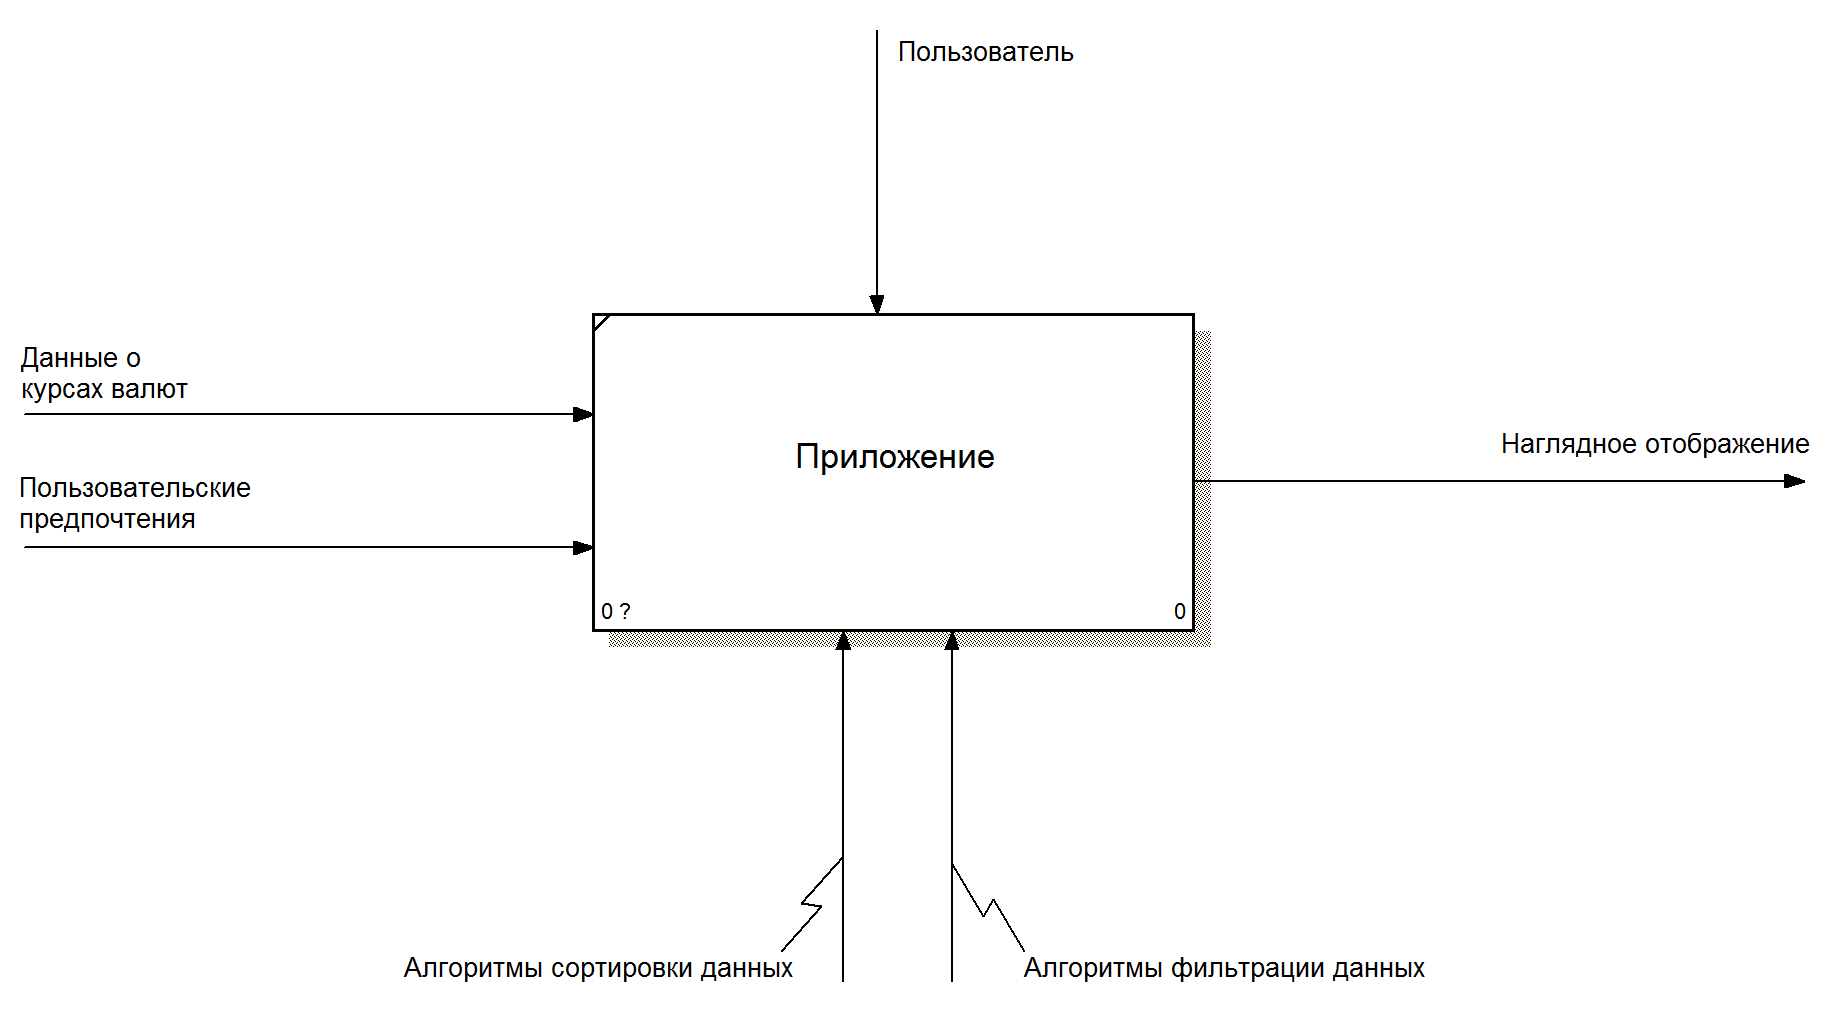
\includegraphics[width=160mm]{fig/IDEF0}
  \caption{Диаграмма декомпозиции \\ верхнего уровня разрабатываемого приложения}
  \label{fig:idef0}
\end{figure}

Из приведенной диаграммы видно, что на вход системе поступают данные
о курсах валют, получаемые с использованием удалённых интерфейсов
прикладного программирования (API): финансового портала myfin.by и официального
сайта Национального банка Республики Беларусь nbrb.by,
а также личные предпочтения пользователя (настройки).
Результатом работы системы являются финансовые данные, прошедшие этапы сортировки,
фильтрации по определенным правилам, управление осуществляет пользователь приложения.

\pagebreak

Рассмотрим подробнее набор входных данных, получаемых от источника myfin.by.
В результате GET-запроса приложение получает данные в формате XML, имеющие вид,
представленный на рисунке~\ref{fig:myfin_input_xml}.
\begin{figure}[h!]
  \centering
  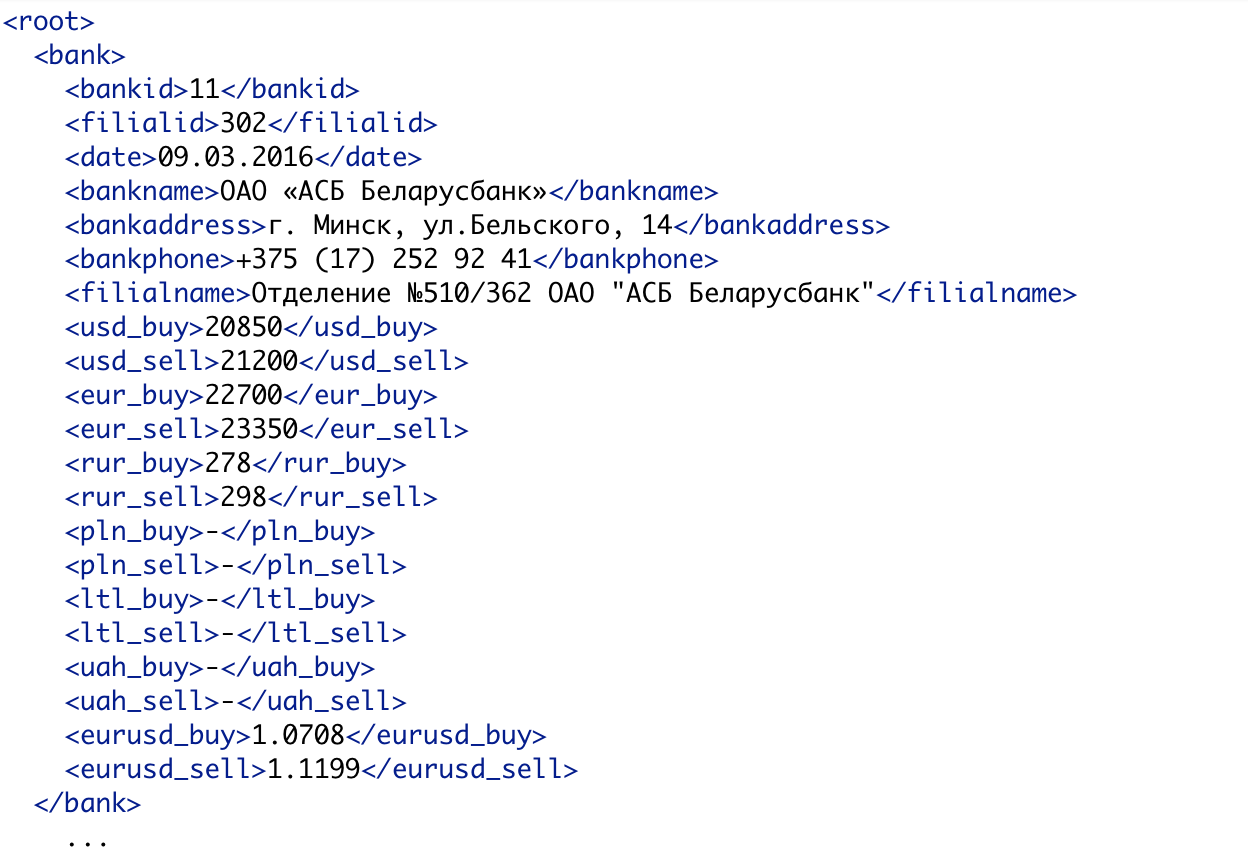
\includegraphics[width=150mm]{fig/myfin_input_xml}
  \caption{Пример входных данных разрабатываемого модуля}
  \label{fig:myfin_input_xml}
\end{figure}

Из приведенного рисунка видно, что информация о конкретном отделении
помещается в тег \textit{bank}. Полноразмерный документ для города Минска
содержит около восьмиста таких объектов, предоставляя адресно-справочную
информацию об отделении банка, а также информацию о курсах валют в нём.

Учитывая большой объём информации, а также требование сохранять полученные данные
на жестком диске устройства для дальнейшего использования в оффлайн-режиме,
необходимость быстрой обработки информации по запросу пользователя
(сортировки, поиска максимальных, минимальных значений, нахождение среднего),
целесообразным является хранение этих данных на устройстве с использованием
мобильной базы данных.

На первый взляд, целесообразным является создание класса \textit{Bank} с полями,
аналогичными полям в XML-документе. Однако при таком подходе мы сталкиваемся с
избыточностью данных. Например, для каждого объекта \textit{bank} во входном
документе есть поле \textit{bankname}, которое будет дублироваться для одного
и того же банка.

С целью решения проблемы избыточности данных, выделим следующие сущности
рассматриваемой предметной области:
\begin{itemize}
  \item банк;
  \item отделение;
  \item курсы валют.
\end{itemize}

Приведенные сущности, а также связи между ними, представлены
на рисунке~\ref{fig:entities}.
\begin{figure}[h!]
  \centering
  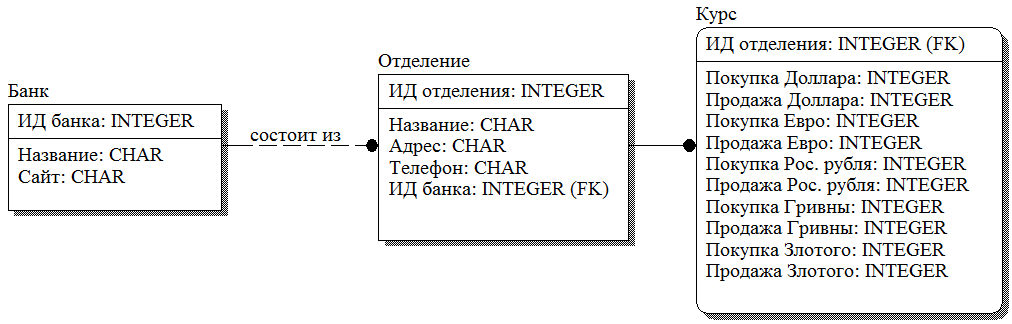
\includegraphics[width=150mm]{fig/entities}
  \caption{Основные сущности предметной области}
  \label{fig:entities}
\end{figure}

Сущность <<Банк>> соответствует общей информации о банке
и состоит из идентификатора, названия и сайта банка.

Сущность <<Отделение>> соответствует информации об отделении банка
и состоит из идентификатора, названия, адреса, телефона, координат.

Сущность <<Курс>> содержит данные о курсах валют.

Сущности <<Банк>> и <<Отделение>> связаны связью
вида один-ко-многим, так как одному банку может соответствовать
множество его дочерних отделений.

Сущность <<Отделение>> и <<Курс>> связаны связью один-к-одному,
так как каждому отделению соответствуют только один набор курсов валют.

Входные данные со стороны Web-сервиса Национального банка Республики Беларусь
представляют собой небольшой XML файл. Учитывая то, что обновление этих данных
происходит на стороне сервера один раз в день, для дальнейшего использования
приложения в оффлайн-режиме будем сохранять эти данные на жесткий
диск устройства в формате XML, загружая информацию в оперативную память
устройства при инициализации приложения.

Выходные данные приложения представляют собой текстовые поля, которые
отображают релевантную финансовую информацию, прошедшую процесс фильтрации
и применения агрегатных функций по определенным правилам.


% Системные требования

\subsection{Системные требования}

Разрабатываемый программный модуль предназначен для использования на устройствах
iPhone любого поколения с установленной операционной системой iOS 8.0 и выше.

Для скачивания программного модуля из магазина приложений
App Store пользователю мобильного устройства необходимо выполнить
вход под единой учётной записью Apple ID. На момент установки приложения на
жестком диске устройства должно быть как минимум 30 Мбайт свободного места.

Для корректной работы приложения во время первого запуска необходимым является
подключение к интернету, с помощью которого устройство загружает актуальную
финансовую информацию с сервера данных.


% Эргономическое обеспечение

\subsection{Эргономическое обеспечение}

Эргономическим обеспечением является совокупность методов и средств,
предназначенных для создания оптимальных условий высокоэффективной и
безошибочной деятельности человека в автоматизированной информационной системе.

Для формирования качеств программного модуля, способных повысить эффективность его
использования, рассмотрим историю развития и совершенствования мобильной
операционной системы iOS.

Руководитель компании Apple Стив Джобс 9 января 2007 года показал на одной
из лучших презентаций компании на выставке-конференции
Macworld Conference \& Expo первый iPhone на базе iPhone OS (совр. iOS).
С того момента прошло больше 7 лет, и многие поколения iPhone, iPod Touch и iPad
кардинально изменили внешнюю оболочку смартфонов и планшетных компьютеров.
Система iOS --— одна из старейших мобильных платформ, однако это не говорит о том,
что в ней не хватает функций, инструментов или же мощности.
Совсем наоборот, корпорация Apple смогла сделать iOS одной из самых функциональных
и поддерживаемых операционных систем, существующих на данный момент.
Каждый год специалисты и разработчики совершенствуют iOS,
о чём говорит увеличивающееся количество пользователей данной мобильной платформы.

Сразу после презентации операционная система iOS не имела многозадачности,
возможности установки сторонних приложений, а также поддержки копирования и вставки.
Однако спустя годы усовершенствованная iOS стала системой такой мощности,
которую можно сравнить с некоторыми компьютерными операционными системами.

В iOS версии 7 компания Apple полностью изменила дизайн,
тем самым задав тенденцию развития интерфейса всех сторонних приложений для этой
платформы на несколько лет вперёд. Директор по дизайну Джонатан Айв описал
обновление как <<внесение порядка в запутанность>>, подчеркивая следующие
особенности новой версии операционной системы: изысканные тонкие шрифты,
прозрачность, слои и новые иконки, дизайн которых не повторяет реальные предметы,
поскольку их назначение понятно интуитивно.
С момента выхода iOS 7 дизайн операционной системы от Apple не претерпел
значительных изменений. Таким образом, Apple продолжает придерживаться
использования тонких шрифтов в дизайне, прозрачных элементом интерфейса,
с каждым обновлением повышая эффективность использования операционной
системы конечным пользователем.

Существенное влияние на развитие операционной
системы от Apple оказал влияние магазин приложений App Store, в котором
любой зарегистрированный разработчик имеет возможность опубликовать своё
приложение. В процессе развития этого магазина приложений компания Apple
создала документ~\cite{ios_hig}, описывающий определённые принципы, которыми следует
руководствоваться при создании приложений. Этот документ описывает общие
правила и рекомендации по расположению основных элементов в приложении,
из размерам, шрифтам текстов и так далее.
Следование этому документу в процессе разработки программного модуля для iOS
гарантирует то, что итоговое приложение будет соответствовать
операционной системе iOS.

До момента выхода iOS версии 9 во всех мобильных устройствах компании Apple
использовалось семейство шрифтов Helvetica Neue. Шрифт Helvetica была
создана в Швейцарии в 1957 году, когда еще не существовало никаких цифровых
устройств. Она, тем не менее, до сих пор используется многими компаниями
в качестве корпоративного шрифта, и, вне всяких сомнений, будет использоваться
и в будущем как хороший классический шрифт.

Шрифт San Francisco, который компания Apple представила на своих устройствах
с версией операционной системы iOS 9, напротив, является современным шрифтом.
Его гарнитура меняется динамически, в соответствии с контекстом.
Его можно назвать своего рода <<родным шрифтом>>
цифровой эпохи~\cite{san_francisco_font}.

Учитывая то, что разрабатываемый программный продукт попадает в категорию <<Финансы>>,
стоит учесть это в выборе цветовой схемы. Очевидно, что пользователь,
выполняющий поиск приложений в этой категории, не захочет просматривать
актуальную финансовую информацию в приложении с пёстрыми цветовым оформлением,
однако и на черно-белое оформление он может просто не обратить внимание.
С учётом этого, в качестве цветовой схемы будем использовать сочетание
тёмно-синего (\#003366), жёлтого (\#003366) и светло-серого (\#003366) цветов.
Вспомогательными цветами являются белый и некоторые оттенки серого цветов.
Используемая цветовая схема разрабатываемого программного модуля
представлена на рисунке~\ref{fig:colors}.
\begin{figure}[h!]
  \centering
  
\includegraphics[width=70mm]{fig/colors}
  \caption{Цветовая схема \\ разрабатываемого программного модуля}
  \label{fig:colors}
\end{figure}

Принимая во внимание то, что шрифт San Francisco соотвествует концепции <<строгий дизайн>>,
при этом являясь стандартным для устройств на платформе iOS,
в рамках разрабатываемого программного модуля следует использовать именного его.
